\chapter{Introduction} \label{chapter1}

%\section{Introduction}

Intrusion Detection Systems (IDSs) have become important tools that help security administrators to identify and analyze unauthorized computer or network activities, from both outsider and insider attacks.
The dominant detection methodologies are signature-based and anomaly-based approaches.
Signature-based (or misuse) IDSs look for events that correspond to patterns of known attacks.
They can provide a high level of accuracy, however are limited to detecting known attacks and vulnerable to polymorphic attacks (which are capable of changing their signatures as they propagate).

Anomaly detection systems (ADSs), on the other hand, monitor for significant deviations from normal system behavior.
They are typically trained (using machine learning and data mining techniques) on datasets collected over a period of attack-free activities to learn the normal system behavior, and then deployed to detect deviations from the expected system behavior.
These deviations are reported as anomalous events, although they are not necessarily malicious activities or attacks because they may also correspond to coding or configuration errors.
An ADS can detect novel attacks (not known during training time) but generate large number of false alarms, because it is difficult to obtain complete descriptions of complex system behavior, which may change over time.

IDSs can also be categorized depending on their location of deployment into network- and host-based detection systems (a more comprehensive taxonomy of IDSs can be found in \cite{Liao2013}).
Network-based IDSs monitor and analyze traffic to and from all devices on the network.
They may be be located anywhere in the network; integrated in network devices (e.g., switches and routers) or as a standalone device.
A host-based IDS runs on a host computer and monitors sensitive activities on this host, such as unauthorized access, modification of files, or system calls.

In this work, we focus on host-based anomaly detection using system calls -- the gateway between user and kernel mode.
Short sequences of system calls have been shown consistent with normal host operation, and can be used to detect attacks \cite{Forrest1996,Warrender1999}.
A large number of research studies have investigated different machine learning and data mining techniques for detecting anomalies in system call sequences \cite{Forrest2008}.
Among these, techniques based on Hidden Markov Models (HMMs)~-- probabilistic models for sequential data~-- have been shown to produce a high level of detection accuracy \cite{Du2004,Gao2002,Hoang2004,Hu2010,Wang2004,Warrender1999,Zhang2003,Khreich2009-ICC, Sultana2012, Murtaza2012}.

The success of an ADS depends largely on the model of normal behavior.
A single HMM may not, however, provide adequate approximation of the underlying data distribution of a complex host system behavior, due to the many local maxima of the likelihood function \cite{Khreich2009-ICC}.
Ensemble methods have been used to improve the overall system accuracy by combining the outputs of several \textit{accurate and diverse} models \cite{Kittler1998,Dietterich2000,Kuncheva2004b,Zhou2012}.
In particular, combining the outputs from multiple HMMs, each trained with a different number of states, in the Receiver Operating Characteristics (ROC) space according to the Iterative Boolean Combination (IBC), has been shown to provide a significant improvement in the detection accuracy of system call anomalies \cite{Khreich2010-ICPR}.

The IBC is a general decision-level combination technique that attempts to select the decision thresholds (from each input detector) and the Boolean functions that maximize the overall ROC convex hull of the combined ensemble \cite{Khreich2010-ICPR}.
As presented in Algorithm~\ref{IBC1}, given $K$ soft detectors that assign scores or probabilities to the input samples, (which can be converted to a crisp detector by setting a threshold on the scores as further detailed in section~\ref{sec:boolean-combination}) , the IBC algorithm starts by combining the outputs of the first two detectors (in the order of input), and then proceeds \textit{sequentially} by combining the resulting combinations with the outputs of third detector, and so on, until the $K^{th}$ detector is combined.
It can then re-iterate to combine the resulting combinations with the original detectors.

The IBC technique provides a practical way for combining relatively large number of detectors while avoiding the exponential explosion of Boolean combinations.
As detailed in Section~\ref{sub:complexity}, applying all Boolean functions using an exhaustive brute-force search to determine optimal combinations leads to an exponential number of combinations, which is prohibitive even for a small number of detectors \cite{Barreno2008}.
Even the \textit{pairwise} Bruteforce Boolean Combination (BBC2), which is used as a baseline reference in our experiments, requires an exponential number of combinations, which is equal to the square of the number of detectors (see Algorithm~\ref{PBC} without the pruning mechanisms).

However, the sequential combinations of soft detectors according to IBC still faces challenges, when a large number of detectors ($K$) is presented for combinations.
First, it produces a sequence of combination rules that grows linearly with $K$ (and the number of iterations), which becomes difficult to analyse and understand.
Furthermore, it makes the algorithm sensitive to the order in which the detectors are input for combinations, which increases the effort required to find best subset for operations.
In any case, combining all available detectors without any pruning mechanism may be inefficient due to the redundancy in their outputs.

In this work, we propose an ADS based on a Pruned Boolean Combination (PBC) algorithm, which employs two novel pruning techniques to select a subset of diverse and accurate detectors for combination, while discarding the remaining ones.
Although both pruning techniques are based on Cohen's Kappa \cite{Cohen1995a} measure, they differ in the way they compute the diversity and accuracy of the selected detectors for combinations.
While the first technique relies only on Kappa measure (MinMax-Kappa), the second uses both Kappa and the ROC convex hull (ROCCH-Kappa).
Therefore, our proposed PBC approach provides an efficient way to prune and combine large number of detectors, which avoids the exponential explosion of combinations of brute-force techniques, and reduces the sequence of combinations provided by IBC.

We evaluate our PBC-based ADS using ADFA Linux Dataset (ADFA-LD)\footnote{http://www.cybersecurity.unsw.adfa.edu.au/ADFA IDS Datasets/}, which has been recently made publicly available on the website of the University of New South Wales \cite{Creech2013a}.
The performance of the PBC using both pruning techniques are compared to that of IBC and BBC2 in terms of ROC analysis and time complexity.
The results show that PBC with both pruning techniques are capable of maintaining similar overall accuracy as measured by the ROC curves to that of IBC and BBC2.
However, the time required for searching and selecting (or pruning) the subset of detectors from the same ensemble of detectors is on average three magnitudes lower for PBC with MinMax-Kappa pruning than that of BBC2.
Furthermore, the experimental results show that PBC with both pruning techniques always provides two crisp detectors for combination (during the operations), while IBC provided an average of $11$ detectors to achieve the same operating point.


\section{System Calls}
\label{sec:system-calls}
A system call is a request in a Unix-like operating system made via a software interrupt by an active process for a service performed by the kernel.
Users' requests are made from higher level applications  to the kernel via a platform-dependent set of system calls. System calls provide an essential interface between a process and the operating system. Applications must invoke system calls to request kernel services, such as access to standard input/output, physical devices and network resources. Every system call has a unique number (known by the kernel) and a set of arguments. Some example of system calls used for file managements is as follows: open(), read(), write(), and close(). System call traces have different lengths that depends on the complexity and execution time of the process.
Manifestations of a wide variety of attacks, including buffer overflows, symbolic link, decode and SYN floods may appear at the system call level and differ from normal behavior of privileged processes, (\cite{Forrest1996}; \cite{Hofmeyr1998}; \cite{Kosoresow1997}; \cite{Somaayaji2002}; \cite{Warrender1999}). Furthermore, after gaining root privileges on a host, attackers will typically try to maintain administrative access on the compromised host (\cite{Mitnick2005}), by for instance installing backdoors and rootkits. Attackers will also attempt to distribute Trojan horses, using for instance comprised email addresses or shared network folders, to compromise other systems. These malicious activities may also invoke different sequences of system calls than those generated during normal execution of a process.

\section{HMM-based Anomaly Detection using System Call Sequences}
\label{sec:ads-hmm}


The temporal order of system calls has been shown consistent with the normal behavior of a privileged process, while an unusual burst will occur during an attack \cite{Forrest1996,Warrender1999}.
The authors proposed a host-based ADS using a simple sequence matching techniques for detecting anomalous system call sequences generated by UNIX privileged processes \cite{Forrest1996}.
System call traces provided for training are first segmented into fixed-length \textit{contiguous} sequences, using a fixed-size sliding window, shifted by one symbol to build the normal profile.
These sequences are then stored in a database that represents the normal process behavior.
During operations, a sliding window (having the same size used to construct the normal profile) to scan the system calls generated by the monitored process for anomalies -- sequences that are not found in the normal database.

Several statistical and machine learning techniques have been investigated over the last two decades for detecting system call anomalies \cite{Forrest2008}.
Application of machine learning techniques include neural network \cite{Ghosh1999}, k-nearest neighbors \cite{Liao2002}, Markov models or n-grams \cite{Jha2001,Marceau2000}, Bayesian models \cite{Kruegel2003a}.
Among these, techniques based on discrete HMMs have been shown to produce a high level of detection accuracy \cite{Warrender1999,Gao2002,Gao2003,Zhang2003,Du2004,Wang2004,Hoang2004,Khreich2009-ICC,Chen2009,Hu2010,Wang2010}.

A discrete HMM is a stochastic process for sequential data \cite{Khreich2012-INS,Rabiner1989}.
An HMM is determined by two interrelated mechanisms -- a latent Markov chain having a finite number of states $N$, and a set of observation probability distributions, each one associated with a state.
 Starting from an initial state $S_{i}\in\{S_{1},...,S_{N}\}$, determined by the initial state probability distribution $\pi_{i}$, at each discrete-time instant, the process transits from state $S_{i}$ to state $S_{j}$ according to the transition probability distribution $a_{ij}$.
The process then emits a symbol $v_{k}$, from a finite alphabet $V=\{v_{1},\ldots,v_{M}\}$ of size $M$ symbols, according to the discrete-output probability distribution $b_{j}(v_{k})$ of the current state $S_{j}$.
HMM is commonly parametrized by $\lambda=(\pi,A,B)$, where the vector $\pi=\{\pi_{i}\}$ is the initial state probability distribution, matrix $A=\{a_{ij}\}$ is the state transition probability distribution, and matrix $B=\{b_{j}(v_{k})\}$ is the state output probability distribution, ($1\leq i,j\leq N$ and $1\leq k\leq M$).
% However, the time and memory complexity for training an HMM with $N$ states according to Baum-Welch algorithm is $\mathcal{O}(N^2T)$ and $\mathcal{O}(NT)$ respectively, for a sequence of length $T$ symbols.

A well trained HMM provides a compact detector that captures the underlying structure of a process based on the temporal order of system calls, and detects deviations from normal system call sequences with high accuracy and tolerance to noise.
Training an HMM from a sequence (or a block) of observation symbols, $o_{1:T}$, aims at estimating HMM parameters $\lambda$ to best fit the training data.
 Typically, parameters estimation consists of maximizing the likelihood of the training data over HMM parameters space, $P(o_{1:T}\mid\lambda)$.
Since this likelihood depends on the latent states, there is no known analytical solution to the learning problem.
Iterative optimization techniques, such as the Baum-Welch (BW) algorithm \cite{Baum1970}, are applied to estimate the HMM parameters over several training iterations, until the likelihood function is maximized.
During operation, the likelihood of a new observation sequence $o_{1:T}$ given a trained HMM $\lambda$, $P(o_{1:T}\mid\lambda)$ is typically evaluated by using the Forward-Backward (FB) algorithm \cite{Khreich2012-INS,Rabiner1989}.
Setting a threshold on the output probabilities of HMM, provides a decision whether the sequence is normal or anomalous.

Few researchers tried to investigate the effect of the number of states on the performance of HMM detectors, and found that $N$ value may have a great impact on the overall performance \cite{Yeung2003,Khreich2009-ICC}.
In particular, combining the outputs from multiple HMMs, each trained with a different $N$ value, in the ROC space according to the IBC technique (as described in the next section), has been shown to provide a significant improvement in the detection accuracy of system call anomalies \cite{Khreich2010-ICPR}.

\section{Anomaly Detection Challenges}
\label{sec:Challenges}
Most works assume being provided with a sufficiently representative amount of clean (attack-free) system call data for training the anomaly detectors, which is not correct most of the time. Even under this assumpotion these techiqnue have some problmes.

Designing and implementing every machine learning algorithms like HMM involves some estimation of parameters like number of hidden states N, initial matrix M. The value of N has a considerable impact not only on system accuracy, but also on HMM training time and memory requirements. The number of states is often chosen heuristically or empirically using validation data. In fact, HMMs trained with different number of states are able to capture different underlying structures of data. Therefore, a single best HMM will not provide a high level of performance over the entire detection space.
The other challenge is the size of the window, every window-based anomaly detection technique using system-call traces in form of window of system calls, the size of window affect performance and accuracy more or less in different technique. The smaller windows size is always desirable since it makes the technique much faster yet we need to have a limit on minimum size in order to be able to detect all of the anomalies \cite{Tan2002}. In general, ADSs are designed to provide accurate results for a particular window size and anomaly size. Discriminative or sequence matching techniques, are only able to detect anomalies with sizes equal to that of the detector window.

As mentioned earlier first and foremost important challenges with anomaly detection techniques are unrepresentative data. in practice is very rare to find a clean data set which represents all of the system behavior so acquiring a sufficient amount of clean data that represents the normal behavior of complex realworld processes is a challenging task. Usually it's not possible to collect all the system behavior and it leads to have an incomplete view of the normal process behavior. Incomplete view of the normal behavior leads to misclassifying rare normal events as anomalous, as illustrated in Figure~\ref{Figure::representative_data}

\begin{figure}[H]
\centering
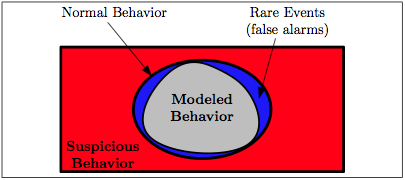
\includegraphics[scale=1]{figs/RepresentativeData}
\caption{Illustration of normal process behavior when modeled with unrepresentative training data. Normal rare events will be considered as anomalous by the ADS, and hence trigger false alarms}
\label{Figure::representative_data}
\end{figure}

Even if there is a way to model and collect all the system behavior system call these behaviors will change over the course of time (either by change of user usage behavior or by changes in monitored environment) and the training model and the clean data set should get updated. 
Changes to the underlying normal distribution lead the model to deviate, and generate both false positive and negative error as illustrated in Figure~\ref{Figure::representative_data_change} Accordingly, the model must be updated from new data to account from this change.


\begin{figure}[H]
\centering
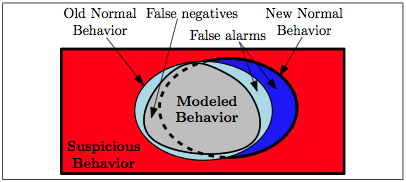
\includegraphics[scale=1]{figs/RepresentativeDataChange}
\caption{Illustration of changes in normal process behavior, due for instance to application update or changes in user behavior, and the resulting regions causing both false positive and negative errors}
\label{Figure::representative_data_change}
\end{figure}

 
